\documentclass[11pt,]{article}
\usepackage[left=1in,top=1in,right=1in,bottom=1in]{geometry}
\newcommand*{\authorfont}{\fontfamily{phv}\selectfont}
\usepackage[]{libertine}


  \usepackage[T1]{fontenc}
  \usepackage[utf8]{inputenc}




\usepackage{abstract}
\renewcommand{\abstractname}{}    % clear the title
\renewcommand{\absnamepos}{empty} % originally center

\renewenvironment{abstract}
 {{%
    \setlength{\leftmargin}{0mm}
    \setlength{\rightmargin}{\leftmargin}%
  }%
  \relax}
 {\endlist}

\makeatletter
\def\@maketitle{%
  \newpage
%  \null
%  \vskip 2em%
%  \begin{center}%
  \let \footnote \thanks
    {\fontsize{18}{20}\selectfont\raggedright  \setlength{\parindent}{0pt} \@title \par}%
}
%\fi
\makeatother




\setcounter{secnumdepth}{0}


\usepackage{graphicx,grffile}
\makeatletter
\def\maxwidth{\ifdim\Gin@nat@width>\linewidth\linewidth\else\Gin@nat@width\fi}
\def\maxheight{\ifdim\Gin@nat@height>\textheight\textheight\else\Gin@nat@height\fi}
\makeatother
% Scale images if necessary, so that they will not overflow the page
% margins by default, and it is still possible to overwrite the defaults
% using explicit options in \includegraphics[width, height, ...]{}
\setkeys{Gin}{width=\maxwidth,height=\maxheight,keepaspectratio}


\title{EnergyScore Bias Research \thanks{Replication files are available
on the author's Github account (\url{http://github.com/Jake-Ford}).
\textbf{Current version}: January 30, 2023; \textbf{Corresponding
author}:
\href{mailto:jake@solstice.us}{\nolinkurl{jake@solstice.us}}.}  }
 



\author{\Large Jacob
Ford\vspace{0.05in} \newline\normalsize\emph{Solstice Power
Technologies}  }


\date{}

\usepackage{titlesec}

\titleformat*{\section}{\normalsize\bfseries}
\titleformat*{\subsection}{\normalsize\itshape}
\titleformat*{\subsubsection}{\normalsize\itshape}
\titleformat*{\paragraph}{\normalsize\itshape}
\titleformat*{\subparagraph}{\normalsize\itshape}


\usepackage{natbib}
\bibliographystyle{apsr}
\usepackage[strings]{underscore} % protect underscores in most circumstances



\newtheorem{hypothesis}{Hypothesis}
\usepackage{setspace}


% set default figure placement to htbp
\makeatletter
\def\fps@figure{htbp}
\makeatother

\usepackage{hyperref}
\usepackage{array}
\usepackage{caption}
\usepackage{graphicx}
\usepackage{siunitx}
\usepackage[table]{xcolor}
\usepackage{multirow}
\usepackage{hhline}
\usepackage{calc}
\usepackage{tabularx}
\usepackage{fontawesome}
\usepackage[para,online,flushleft]{threeparttable}
\usepackage{float}
\floatplacement{figure}{H}
\usepackage{booktabs}
\usepackage{longtable}
\usepackage{array}
\usepackage{multirow}
\usepackage{wrapfig}
\usepackage{float}
\usepackage{colortbl}
\usepackage{pdflscape}
\usepackage{tabu}
\usepackage{threeparttable}
\usepackage{threeparttablex}
\usepackage[normalem]{ulem}
\usepackage{makecell}
\usepackage{xcolor}

% move the hyperref stuff down here, after header-includes, to allow for - \usepackage{hyperref}

\makeatletter
\@ifpackageloaded{hyperref}{}{%
\ifxetex
  \PassOptionsToPackage{hyphens}{url}\usepackage[setpagesize=false, % page size defined by xetex
              unicode=false, % unicode breaks when used with xetex
              xetex]{hyperref}
\else
  \PassOptionsToPackage{hyphens}{url}\usepackage[draft,unicode=true]{hyperref}
\fi
}

\@ifpackageloaded{color}{
    \PassOptionsToPackage{usenames,dvipsnames}{color}
}{%
    \usepackage[usenames,dvipsnames]{color}
}
\makeatother
\hypersetup{breaklinks=true,
            bookmarks=true,
            pdfauthor={Jacob Ford (Solstice Power Technologies)},
             pdfkeywords = {bias, machine learning, equal
opportunity},  
            pdftitle={EnergyScore Bias Research},
            colorlinks=true,
            citecolor=blue,
            urlcolor=blue,
            linkcolor=magenta,
            pdfborder={0 0 0}}
\urlstyle{same}  % don't use monospace font for urls

% Add an option for endnotes. -----


% add tightlist ----------
\providecommand{\tightlist}{%
\setlength{\itemsep}{0pt}\setlength{\parskip}{0pt}}

% add some other packages ----------

% \usepackage{multicol}
% This should regulate where figures float
% See: https://tex.stackexchange.com/questions/2275/keeping-tables-figures-close-to-where-they-are-mentioned
\usepackage[section]{placeins}


\begin{document}
	
% \pagenumbering{arabic}% resets `page` counter to 1 
%    

% \maketitle

{% \usefont{T1}{pnc}{m}{n}
\setlength{\parindent}{0pt}
\thispagestyle{plain}
{\fontsize{18}{20}\selectfont\raggedright 
\maketitle  % title \par  

}

{
   \vskip 13.5pt\relax \normalsize\fontsize{11}{12} 
\textbf{\authorfont Jacob Ford} \hskip 15pt \emph{\small Solstice Power
Technologies}   

}

}








\begin{abstract}

    \hbox{\vrule height .2pt width 39.14pc}

    \vskip 8.5pt % \small 

\noindent Using data on over 800,000 utility payment performance
records, we apply quantitative measurements previously identified to
measure bias in classification algorithms and consider additional
protected classes previously lacking attention, including race, income,
home ownership status, and education levels. We find that relative to
FICO scores, variance in a machine learning model for most scenarios
considered.


\vskip 8.5pt \noindent \emph{Keywords}: bias, machine learning, equal
opportunity \par

    \hbox{\vrule height .2pt width 39.14pc}



\end{abstract}


\vskip -8.5pt


 % removetitleabstract

\noindent  

\hypertarget{introduction}{%
\section{Introduction}\label{introduction}}

As the use of machine learning algorithms continues to spread across
industries, concerns about the potential for these algorithms to amplify
existing biases have become increasingly relevant. To address this,
various techniques for measuring and mitigating bias in machine learning
models have been developed. This case study focuses on evaluating the
level of bias within a risk assessment algorithm and comparing it to the
traditional credit score model. The study employs the algorithmic
fairness definitions put forth by \citet{DBLP:journals/corr/HardtPS16}
and aims to achieve two objectives: first, to assess the level of bias
using traditional fairness criteria and second, to conduct a novel
analysis by extending the number of protected classes considered. The
results of this study will provide a quantitative comparison of the
degree of discrimination faced by different protected classes in this
specific use case.

\hypertarget{related-work}{%
\subsection{Related Work}\label{related-work}}

Fairness through unawareness, an approach to race-neutral threshold
setting in multiple industries, has been widely criticized for being
ineffective. \citet{DBLP:journals/corr/abs-1104-3913}. argue that
researchers should embrace protected classes in the data to achieve a
more accurate analysis of fairness. A similarity metric is used to
describe the degree of similarity between individuals or groups, thereby
revealing the ground truth of the distribution of the protected class.
However, cases where protected class data is unavailable are not
considered in this review.

Similarly, \citet{pmlr-v28-zemel13} acknowledge that bias cannot be
completely eliminated from data or models, and that machine learning
systems trained on historical data will inevitably inherit past biases.
To address this, the authors propose a new algorithm that maps
individuals to a probability distribution while preserving as much
information as possible, while minimizing loss of identifiable
information. The results of this algorithm show improved accuracy and
significant fairness, as measured by both individual and group
definitions, compared to comparison models.

Furthermore, a recent study \citet{DBLP:journals/corr/abs-1901-10002}
highlights the importance of considering the entire life cycle of
machine learning analysis to understand and mitigate sources of bias.
The authors argue that blaming unfair results on biased data
oversimplifies the complex processes involved in collecting, cleaning,
processing, and modeling the data. These processes involve multiple
human decisions that can collectively contribute to unintended results.
The authors aim to increase awareness and focus on the cumulative
sources of bias in machine learning, leading to the development of
mitigation techniques.

\hypertarget{energyscore}{%
\subsection{EnergyScore}\label{energyscore}}

The machine learning algorithm, EnergyScore, has previously been
described by \citet{NBERw26178}. I employ the original dataset used to
create EnergyScore. To allow for an analysis of protected classes and to
avoid data leakage, I use the training datset to construct and re-train
the model, using the test dataset to quantify the effects on different
protected classes.

EnergyScore was shown to be a more inclusive and accurate predictor of
utility bill payment performance than a traditional credit score. This
research will determine the extent to how different protected classes
face discriminatory thresholds, using EnergyScore as the treatment
compared to the tradiitionally used credit score.

\hypertarget{methods}{%
\section{Methods}\label{methods}}

\hypertarget{data}{%
\subsection{Data}\label{data}}

The machine learning model analyzed in this study is EnergyScore, a
patent-pending risk assessment tool designed as an alternative to
traditional credit scores. Previous work has shown the increase in
overall accuracy and inclusion, particularly for low-to-moderate (LMI)
populations \citet{NBERw26178}.

This study uses the data used to train EnergyScore. Account-level credit
account data collected between December 2009 and November 2016. Overall,
over 800,000 observations of utility payment performance were collected
across all fifty states and the District of Columbia. Credit history
data, including FICO scores but also related utility payment performance
history, was included as input variables.

\hypertarget{descriptive-statistics}{%
\subsection{Descriptive Statistics}\label{descriptive-statistics}}

Summary statistics are presented below in Table \ref{tab:desctab} for
the four relevant variables used in this analysis: race, home ownership,
education and race. Totals may not equal due to missing data. Notably,
race suffers from a large degree of data marked as `other', comprising
91.6\% of the total. This category was dropped in the threshold analysis
in the `Results' section, so is not reported here.

\begin{table}

\caption{\label{tab:desctab}Descriptive Statistics}
\centering
\begin{tabu} to \linewidth {>{\raggedright}X>{\raggedleft}X>{\raggedright}X>{\raggedleft}X>{\raggedleft}X}
\hline
Variable & N & Frequency & Average FICO & Late Payment \%\\
\hline
\multicolumn{5}{l}{\textbf{Late Payment}}\\
\hline
\hspace{1em}Late & 304,836 & 34.9\% & 452.587 & NA\\
\hline
\hspace{1em}Not Late & 567,420 & 65.1\% & 733.680 & NA\\
\hline
\multicolumn{5}{l}{\textbf{Race}}\\
\hline
\hspace{1em}Asian & 464 & 1.8\% & 664.759 & 0.291\\
\hline
\hspace{1em}Black & 7,625 & 29.3\% & 548.416 & 0.662\\
\hline
\hspace{1em}Hispanic & 6,118 & 23.5\% & 666.046 & 0.254\\
\hline
\hspace{1em}White & 11,850 & 45.5\% & 602.321 & 0.538\\
\hline
\multicolumn{5}{l}{\textbf{Home Ownershp}}\\
\hline
\hspace{1em}Own & 675,017 & 77.4\% & 667.555 & 0.265\\
\hline
\hspace{1em}Rent & 197,137 & 22.6\% & 525.558 & 0.638\\
\hline
\multicolumn{5}{l}{\textbf{Income}}\\
\hline
\hspace{1em}Low & 270,417 & 31\% & 712.349 & 0.170\\
\hline
\hspace{1em}Medium & 285,222 & 32.7\% & 550.488 & 0.546\\
\hline
\multicolumn{5}{l}{\textbf{Education}}\\
\hline
\hspace{1em}High & 316,515 & 36.3\% & 646.337 & 0.326\\
\hline
\hspace{1em}College & 182,783 & 21\% & 681.666 & 0.226\\
\hline
\hspace{1em}Graduate School & 97,746 & 11.2\% & 702.509 & 0.184\\
\hline
\hspace{1em}High School & 587,566 & 67.4\% & 609.634 & 0.416\\
\hline
\hspace{1em}Vocational/Technical & 4,059 & 0.5\% & 678.342 & 0.204\\
\hline
\end{tabu}
\end{table}

To more accurately and inclusively quantify risk, several regression and
machine learning algorithms were trained to predict risk of default
payment. The best performing model was a random forest construction,
which recorded the highest accuracy scores. This model also produced
higher profits for lenders, as the EnergyScore provides a much more
holistic metric on an individual's ability to pay utility bills. This
better captures those individuals who would have been rejected due to
lower FICO scores but able to pay (false negatives) while minimizing
those who would have been accepted and failed to pay (false positives).
Finally, the EnergyScore increases access for LMI customers, as an
increase in both effectiveness for a larger applicant pool and an
efficient manner of quantifying risk of late payment.

Case studies are useful illustrations of levels of bias measurable in
machine learning applications. This research follows the approach of
\citet{DBLP:journals/corr/HardtPS16}, building upon their work in two
distinct areas. First, we compare bias measurements for the machine
learning algorithm (EnergyScore) and the counterfactual where credit
scores are applied. Secondly, we extend the analysis across multiple
protected classes; including race, income, education and homeownership
status.

\hypertarget{bias-measurements}{%
\subsection{Bias Measurements}\label{bias-measurements}}

Quantitative measurements of bias and fairness are provided for both
EnergyScore and the comparison FICO score. Bias will be measured by
disparate effects on sub-groups in threshold scenarios. Additionally,
the threshold scenarios can be completed by optimizing either FICO
scores or EnergyScore. For simplicity, FICO scores are first used in the
scenarios, EnergyScore will next be used. This will allow both a
baseline observation of how both metrics perform at bias measurements,
and a comparison to determine how EnergyScore performs in fairness
measurements compared to FICO cutoffs.

Using the methodology designed by \citet{DBLP:journals/corr/HardtPS16},
the following scenarios will be applied to our protected classes:

\hypertarget{profit-maximization}{%
\subsubsection{Profit Maximization}\label{profit-maximization}}

Maximum Profits assumes that lenders will seek to minimize false
positives. Hence, a cutoff for applicants is required. A FICO cutoff of
620 is used for good credit as classified by the Consumer Financial
Protection Bureau. From the Non-default rate/FICO score graph below,
setting the setting the FICO score to 620 results in the \emph{total}
non-default rate of 59\%; or the default rate to 41\%. Hence, for profit
maximization we will set the FICO scores accordingly so that each group
achieves maximum 41\% default rate. Notice how from the graph below,
individual FICO cutoffs will differ widely, Hispanics having the lowest
and Whites having the highest.

To arrive at the EnergyScore threshold, the computation includes
analyzing the share of the group approved, then setting the EnergyScore
threshold to the same proportion. This concept is seen in the idea of
demographic parity, and was taken from the EnergyScore
\href{https://solstice.us/wp-content/uploads/EnergyScore-White-Paper-1.pdf}{whitepaper}.

\begin{figure}
\centering
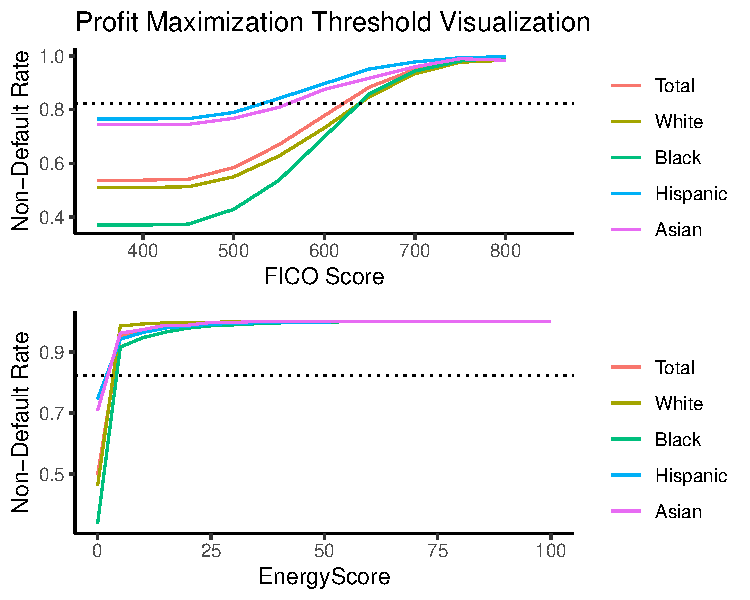
\includegraphics{figs/profitmax.pdf}
\caption{\label{fig:profitmax}Profit Maximization Threshold}
\end{figure}

In Figure \ref{fig:profitmax} we see the non-default rates plotted with
various levels of FICO threshold cutoffs. To arrive at the EnergyScore
threshold, the computation includes analyzing the share of the
groupapproved, then setting the EnergyScore threshold to the same
proportion.

\hypertarget{race-blind}{%
\subsubsection{Race Blind}\label{race-blind}}

Similar to maximum profits, but only apply single threshold to all
groups; hence all groups will be applied the same threshold of 620 for
FICO. Hence, in threshold comparison section at end of each group, no
variation will be observed.

\hypertarget{demographic-parity}{%
\subsubsection{Demographic Parity}\label{demographic-parity}}

This theory sets the thresholds different for each group such that the
proportion of accepted is equal across all groups. This leads to
divergent thresholds per group. The graph below shows the same
cumulative distribution curves. In demographic parity constraints, the
threshold is calculated by setting the proportion of population above
that valye. Figure \ref{fig:demparity} below visualizes the result, as
different subgroups, race in this instance, would receive different
thresholds.

\begin{figure}
\centering
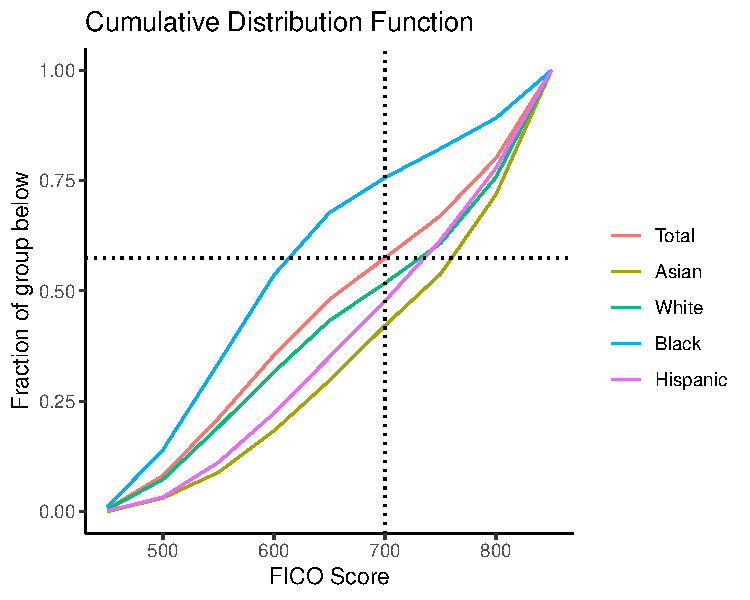
\includegraphics{figs/demparity.pdf}
\caption{\label{fig:demparity}Demographic Parity Threshold}
\end{figure}

\hypertarget{equal-opportunity}{%
\subsubsection{Equal Opportunity}\label{equal-opportunity}}

The true positive rate in data science field refers to the proportion of
those approved by a threshold who do not default; i.e.~the true paying
individuals who are approved. Hence, this criteria sets the true
positive rate equal across all groups. In the graph below, the true
positive rate is shown with varying levels of FICO score cutoffs. In the
example, the developer would choose a true positive level, in the below
70\%, and apply the varying thresholds accordingly.

\begin{figure}
\centering
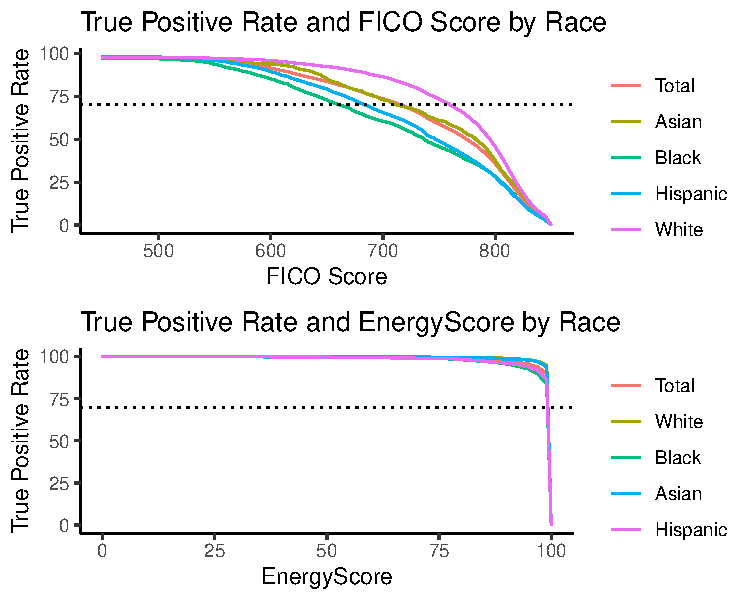
\includegraphics{figs/equalop.pdf}
\caption{\label{fig:equalop}Equal Opportunity Threshold}
\end{figure}

\hypertarget{results}{%
\section{Results}\label{results}}

To quantify how the four protected classes of interest are treated under
the four threshold construction scenarios, we provide the following
results. First, the thresholds for each protected class are shown on a
continuum of the respective metrics range. This shows the relative
difference in treatments within a particular metric.

Secondly, Intra-Group percentiles are shown to compare how individuals
within a particular protected class are treated within the four
threshold scenarios. For example, in Figure \ref{fig:intra} the
percentile value of the threshold is graphed. This second finding
critically shows how individual protected classes are treated
differently between the threshold scenarios.

Finally, the false positive curves are plotted. These visualize the
predictive accuracy of the respective metric, particularly relevant here
for organizations extending credit opportunities, as these examples
represent errant approvals with associated losses.

\hypertarget{thresholds}{%
\subsection{Thresholds}\label{thresholds}}

In Figure \ref{fig:fpfig1} the thresholds are shown for Income and Race.

\begin{figure}
\centering
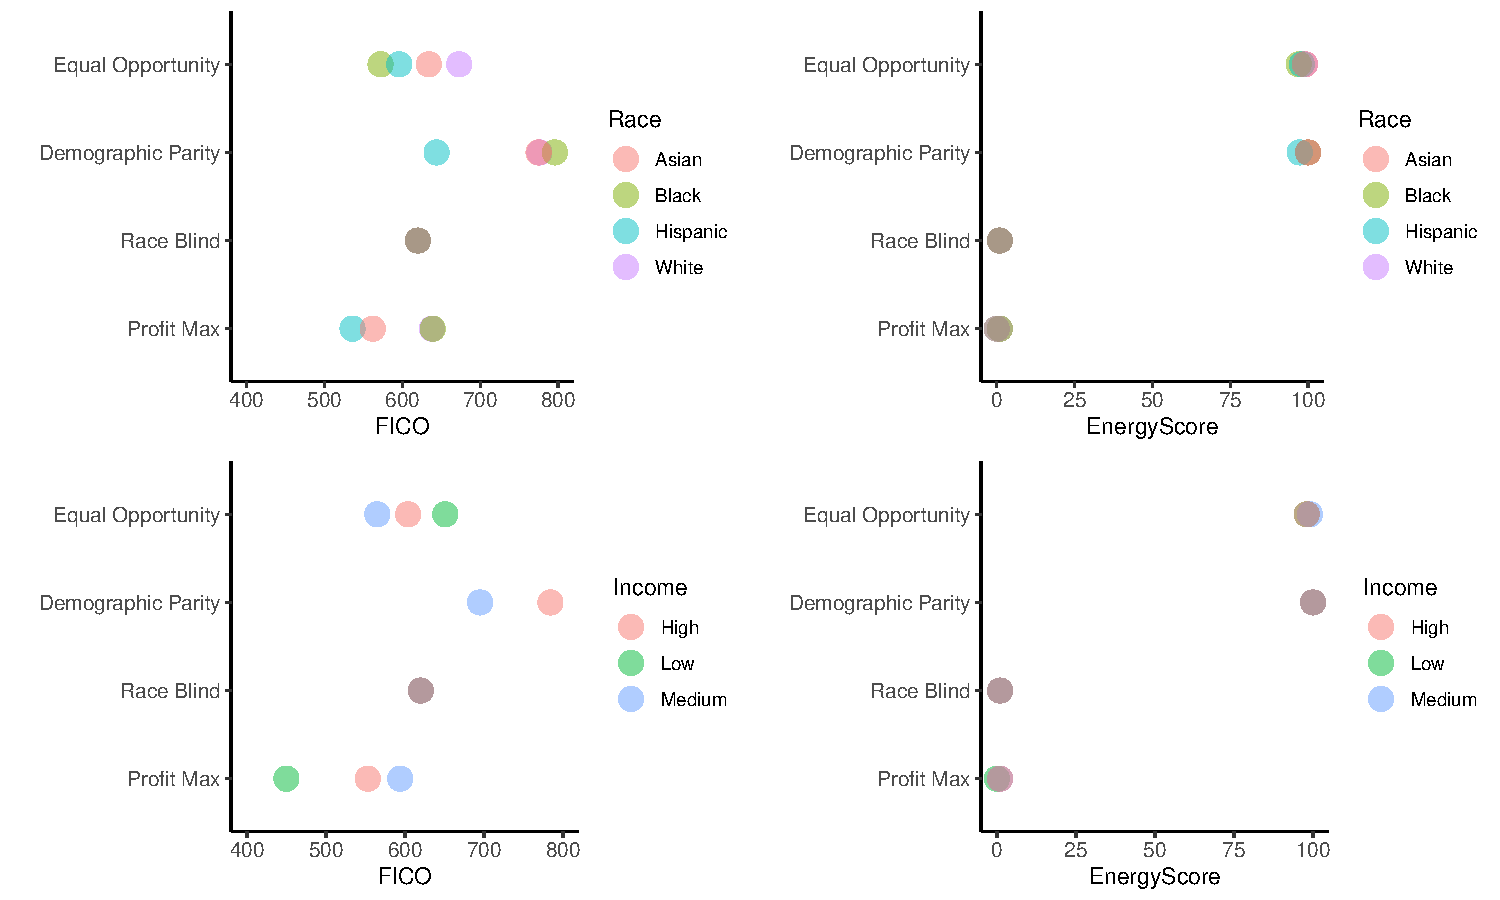
\includegraphics{figs/fpfig1.pdf}
\caption{\label{fig:fpfig1}False Positive Comparison}
\end{figure}

In Figure \ref{fig:fpfig2} the thresholds are shown for Education and
Homeownership.

\begin{figure}
\centering
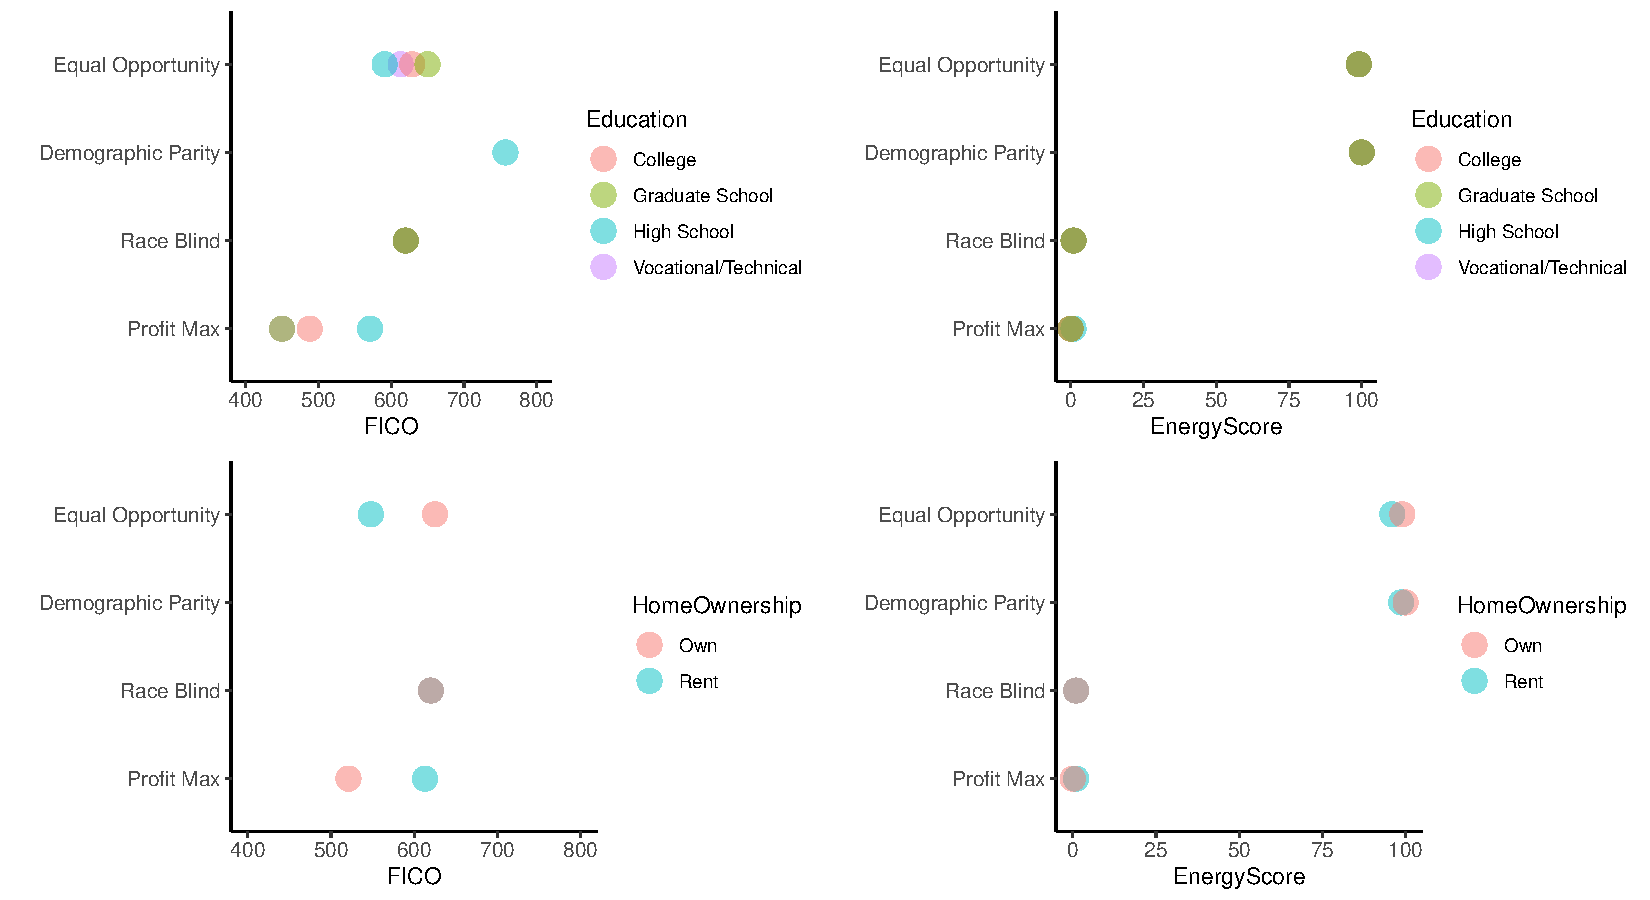
\includegraphics{figs/fpfig2.pdf}
\caption{\label{fig:fpfig2}False Positive Comparison Continued}
\end{figure}

\hypertarget{intra-group-percentiles}{%
\subsection{Intra Group Percentiles}\label{intra-group-percentiles}}

\begin{figure}
\centering
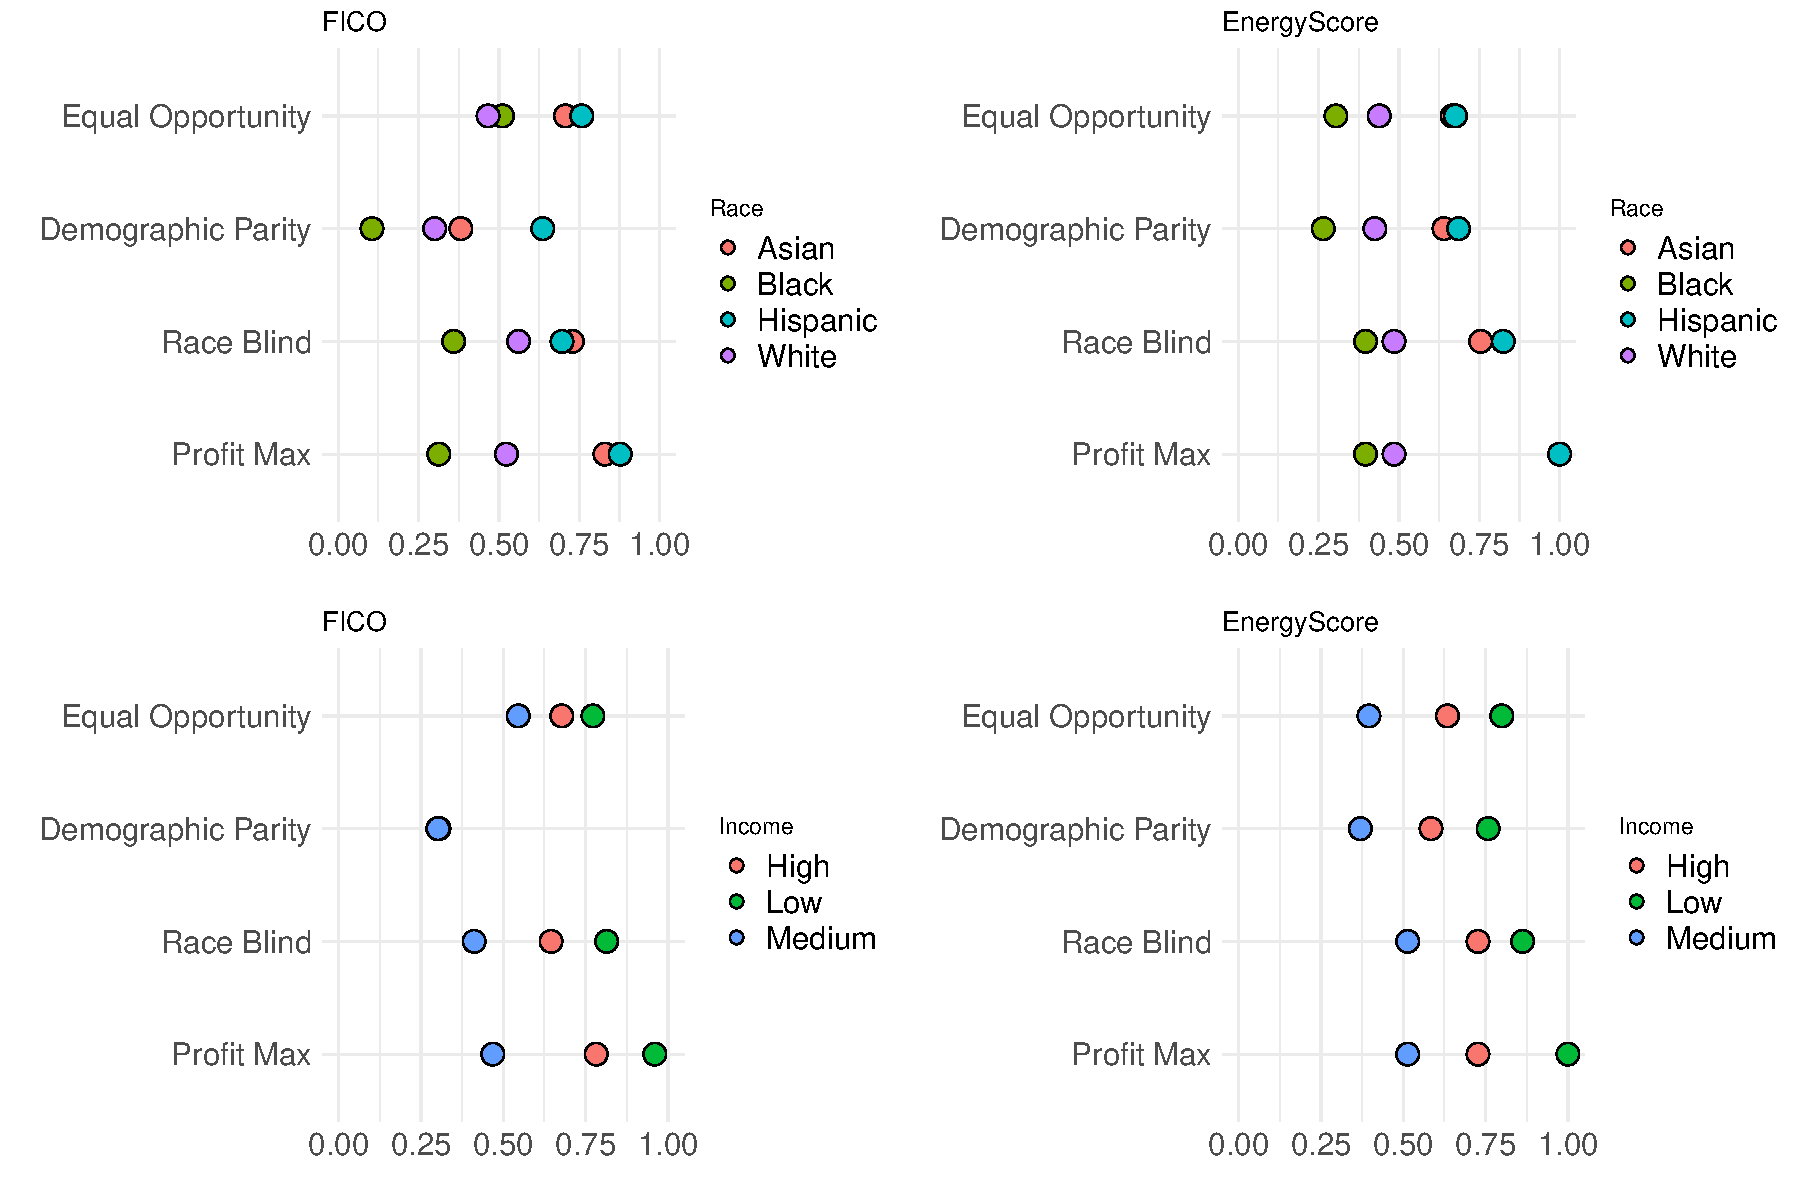
\includegraphics{figs/intra.pdf}
\caption{\label{fig:intra}Intra-Group Percentiles Comparison}
\end{figure}

\begin{figure}
\centering
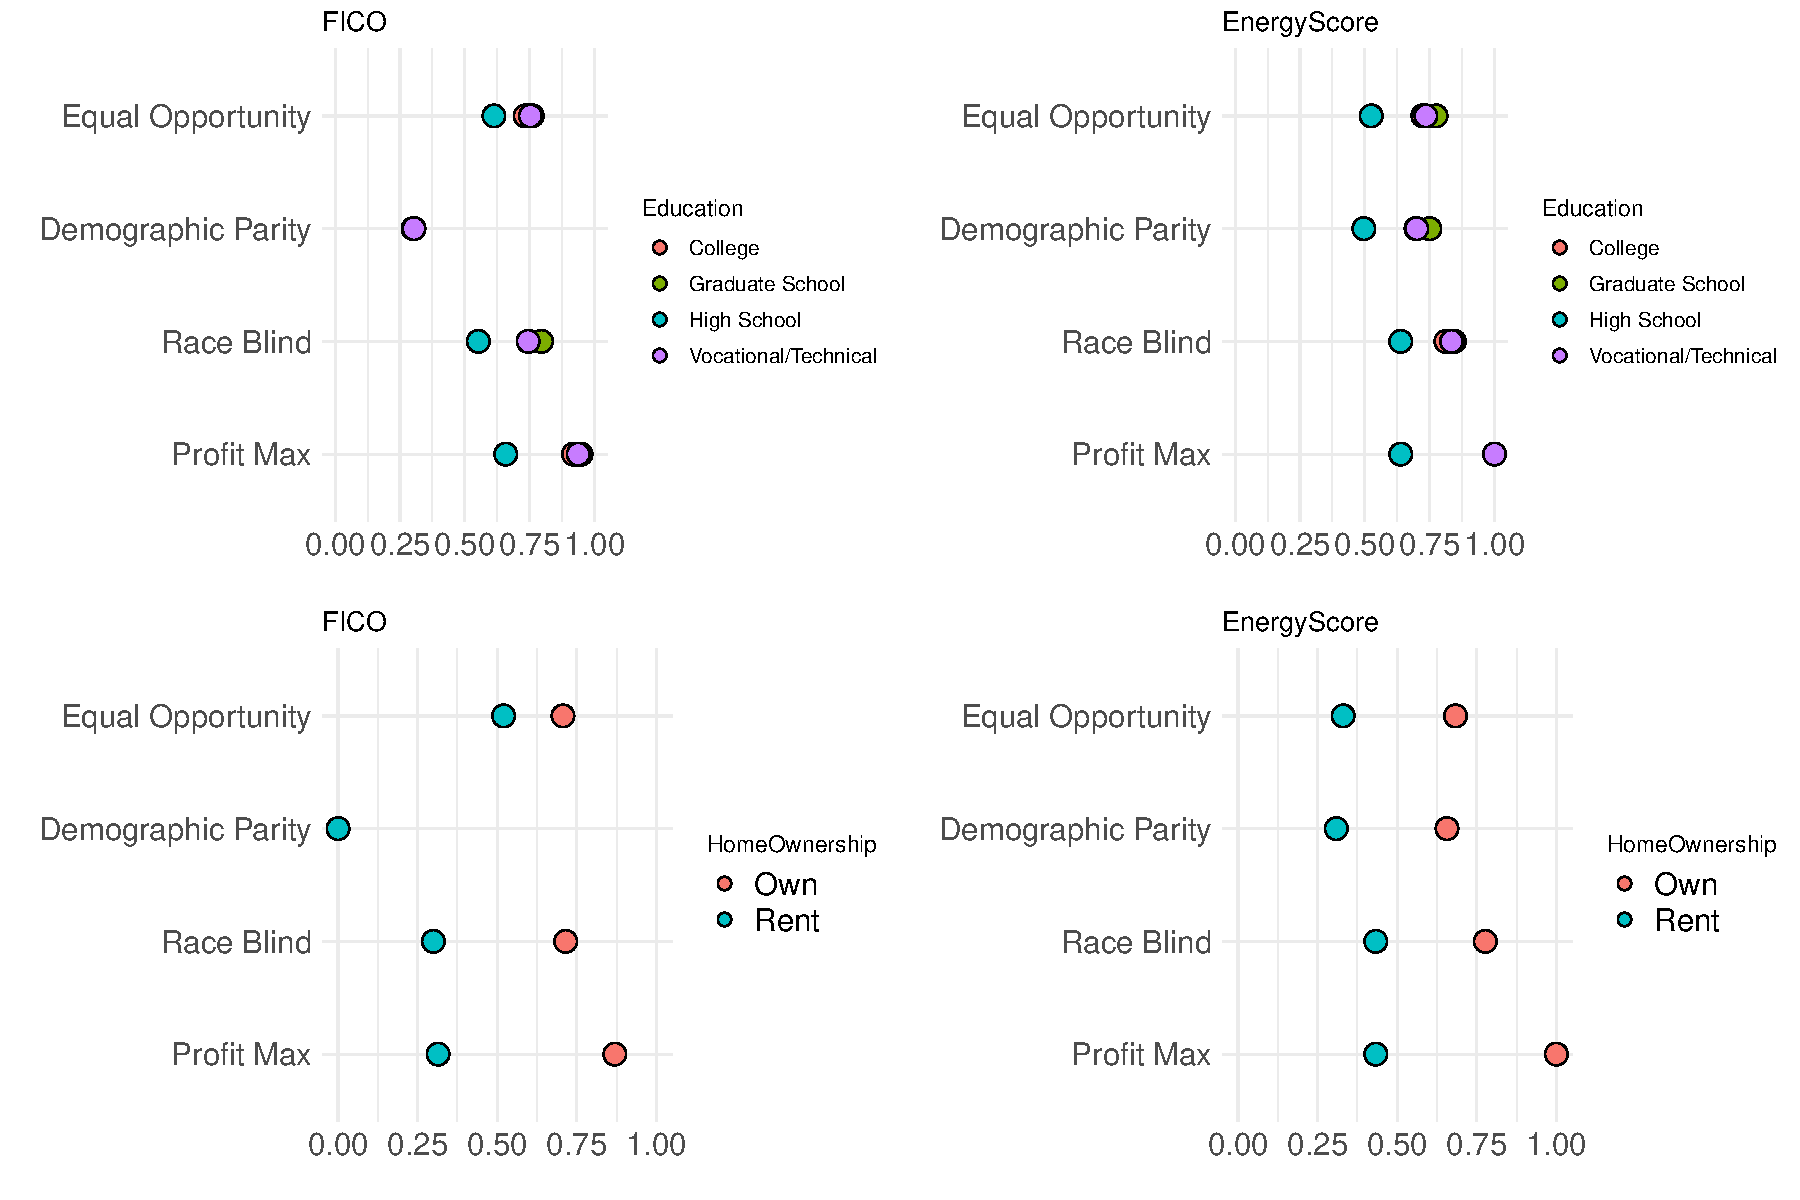
\includegraphics{figs/intra2.pdf}
\caption{\label{fig:intra2}Intra-Group Percentiles Comparison Continued}
\end{figure}

\hypertarget{false-positive-comparisons}{%
\subsection{False Positive
Comparisons}\label{false-positive-comparisons}}

In Figure \ref{fig:fprace} the false positives are shown for Race and
Income

\begin{figure}
\centering
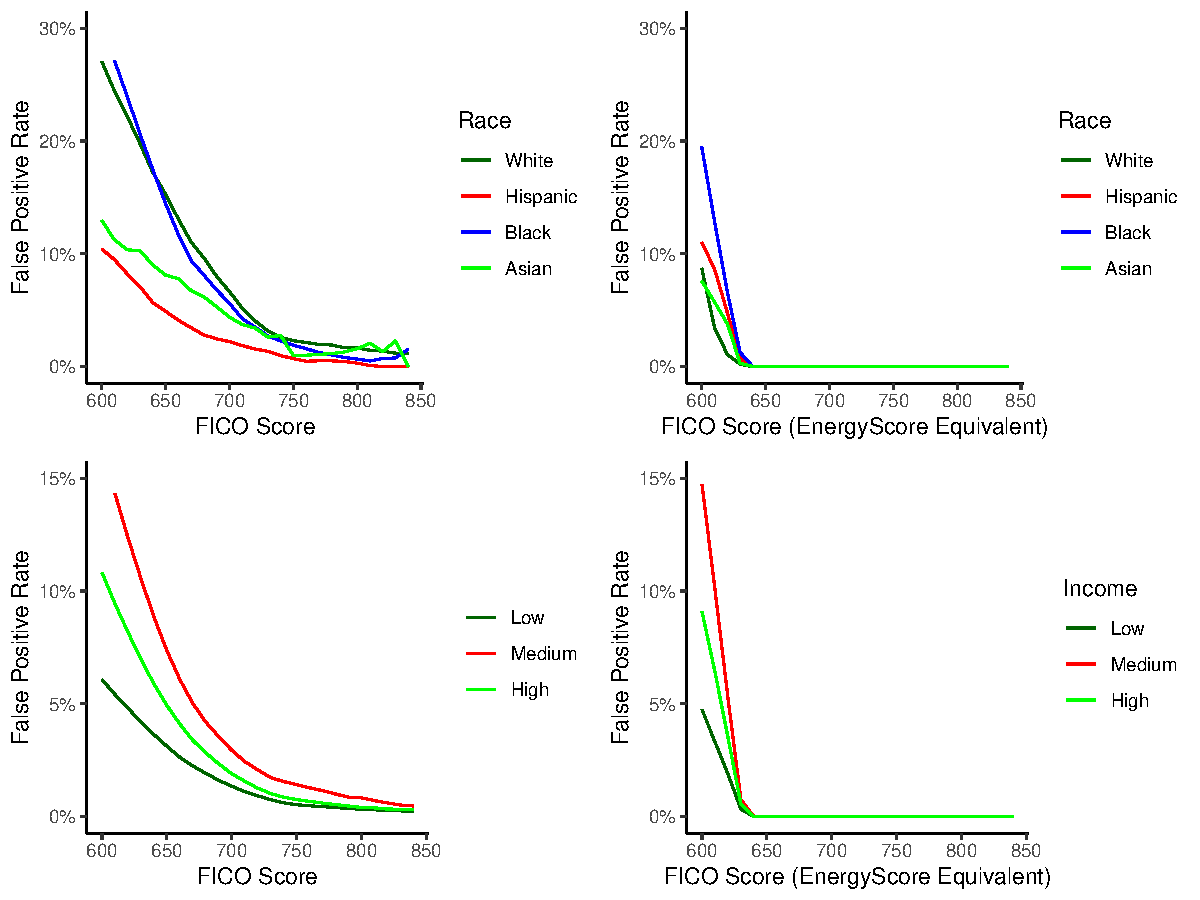
\includegraphics{figs/fprace.pdf}
\caption{\label{fig:fprace}False Positive Comparison}
\end{figure}

In Figure \ref{fig:fprace2} the false positives are shown for Race and
Income

\begin{figure}
\centering
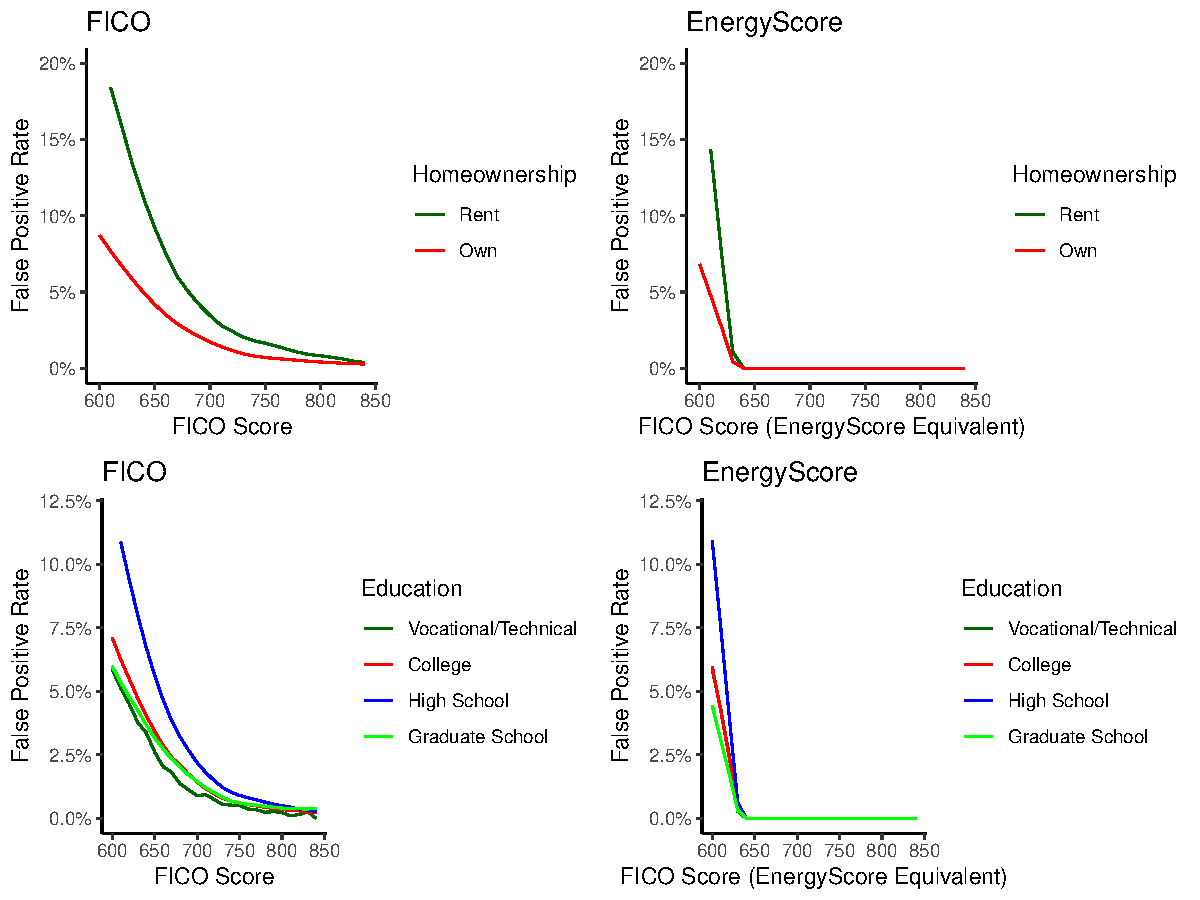
\includegraphics{figs/fprace2.pdf}
\caption{\label{fig:fprace2}False Positive Comparison, Continued}
\end{figure}

\hypertarget{funding}{%
\section{Funding}\label{funding}}

This work was supported by the Tides Foundation grant TF2112-104450.

\hypertarget{data-availability}{%
\section{Data Availability}\label{data-availability}}

The datasets generated and/or analyzed during this study are not
publicly available as they include information relating to a pending
patent application.





\newpage
\singlespacing 
\bibliography{master.bib}

\end{document}
